\documentclass[11pt, oneside]{article}   	% use "amsart" instead of "article" for AMSLaTeX format
\usepackage{geometry}                		% See geometry.pdf to learn the layout options. There are lots.
\geometry{letterpaper}                   		% ... or a4paper or a5paper or ... 
%\geometry{landscape}                		% Activate for for rotated page geometry
%\usepackage[parfill]{parskip}    		% Activate to begin paragraphs with an empty line rather than an indent
\usepackage{graphicx}				% Use pdf, png, jpg, or eps� with pdflatex; use eps in DVI mode
								% TeX will automatically convert eps --> pdf in pdflatex		
\usepackage{amssymb}
\usepackage{amsmath}
\usepackage{parskip}
\usepackage{color}
\usepackage{hyperref}

\title{Introduction to Fourier series}
%\author{The Author}
%\section{}
%\subsection*{}
\date{}							% Activate to display a given date or no date

\graphicspath{{/Users/telliott_admin/Dropbox/Tex/png/}}
% \begin{center} 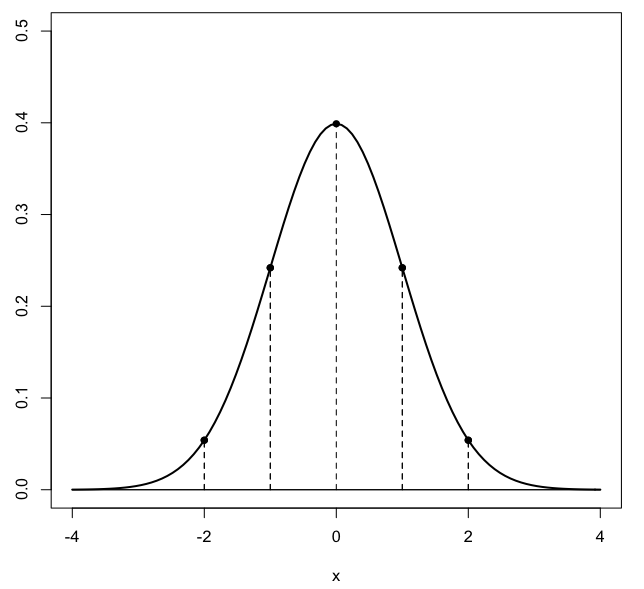
\includegraphics [scale=0.4] {gauss3.png} \end{center}
\begin{document}
\maketitle
\Large
Before we start manipulating equations, let's just look at some plots.  Here are the sine and cosine (from $x=-\pi \rightarrow \pi$).
\begin{center} 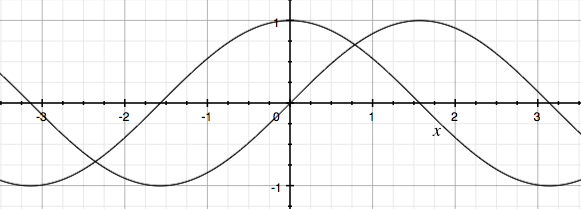
\includegraphics [scale=0.5] {fourier_intro1.png} \end{center}
It's clear by inspection that because of its rotational symmetry as an odd function ($f(-x) = -f(x)$), when the sine curve is integrated \emph{between any limits} $-L \rightarrow L$, we obtain zero total area.

On the other hand the cosine is an even function and the integral from $-L \rightarrow 0$ is equal to the integral from $0 \rightarrow L$.  Depending on where $L$ is placed, the total area may be positive, zero, or even less than zero.  In particular, the area is zero for $-\pi \rightarrow 0$, for $x=0 \rightarrow \pi$ or for the sum of the two intervals.

The second point is to see clearly what happens to $\cos kx$ for $k \in \{1,2,3 \dots \}$.  In the figure below, the function $\cos 4x$ makes four complete cycles in the time that $\cos x$ makes one.  Also, since $4$ is even, $\cos 4 \pi = \cos 2 \pi = \cos 0 = 1$, while $\cos \pi = -1$.  The integral is $0$ over its period $\pi/4$, or any multiple.  In fact, one can start at any point $x=a$ and go till $\rightarrow x=a + T$ where $T$ is the period, and the integral will be zero.  The same is true for the sine.

\begin{center} 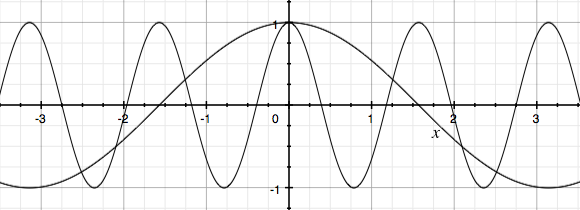
\includegraphics [scale=0.5] {fourier_intro2.png} \end{center}

The next thing is to look at products of functions.  Here are $\cos^2 x$ and $\cos^2 4x$.
\begin{center} 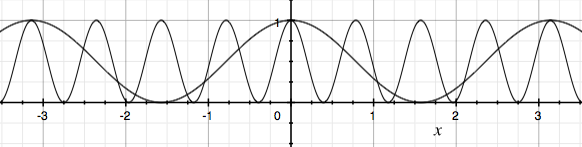
\includegraphics [scale=0.5] {fourier_intro3.png} \end{center}
It seems clear that any function $\cos kx$ squared is an even function.  So the integral over any interval $x=-L \rightarrow 0$ is equal to the integral over the interval $x=0 \rightarrow L$, and in particular, the integral from $x=-\pi \rightarrow \pi$ is non-zero.

Now look at the product $\cos x \cos 4x$, compared to cosine squared.
\begin{center} 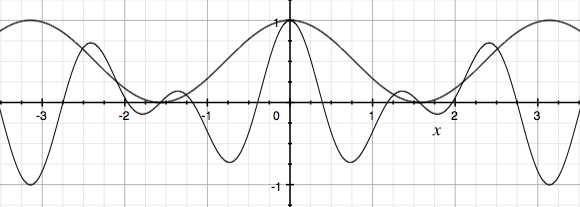
\includegraphics [scale=0.5] {fourier_intro4.png} \end{center}
This function is symmetric across the $x$-axis over the interval $x=0 \rightarrow x=\pi$, and the integral from $x=-\pi \rightarrow \pi$ is zero, as is the integral from $0 \rightarrow \pi$.  In fact any limits symmetric with respect to $\pi/2$ will give zero area.

\begin{center} 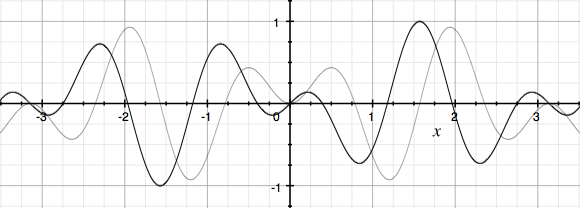
\includegraphics [scale=0.5] {fourier_intro5.png} \end{center}
Finally, here are $\sin x \cos 4x$ (bold) and $\sin x \sin 4x$.  The product of sine and cosine is rotationally symmetric, so the integral from any $x=-L \rightarrow L$ is equal to zero (the product of an even function and an odd function is an odd function).  On the other hand $\sin x \sin 4x$ is an even function.  But it also has the important property that for a suitable period ($\pi$), the negative area balances the positive area and the integral is equal to zero.

If you're getting the idea that lots of these integrals are zero, especially over a suitable interval, then you are on the right track.

\subsection*{cosine times cosine}
For all of these examples, the limits of integration will be $x=-\pi \rightarrow \pi$.  We'll consider other intervals later.
\[ \int_{-\pi}^{\pi} \cos mx \cos nx \ dx;  \ \ n,m \in \{0,1,2 \dots \} \]
For this one, we recall the formulas for sum and difference of cosine, and add the two together.  The $\sin s \sin t$ terms cancel, and we're left with
\[ \cos s + t + \cos s - t = 2 \cos s \cos t \]
Therefore
\[ \int_{-\pi}^{\pi} \cos mx \cos nx \ dx \]
\[ = \frac{1}{2} \int_{-\pi}^{\pi} \cos (m+n) x + \cos (m-n) x \ dx \]
\[ =  \frac{1}{2} \ [ \ \frac{\sin (m+n) x}{m+n} + \frac{\sin (m-n) x}{m-n} \ ] \]
In the case where $m \ne n$ and $m$ and $n$ are both non-zero, we have two terms with $\sin kx$, but for any integer $k$, $\sin kx = 0$.

In the case where $m=n=0$ or $m=n\ne 0$ we would have division by zero, but looking at the integral, both of the functions being integrated are equal to $\cos(0)=1$, so we're OK.

For $m=n=0$, the result is 
\[ = \frac{1}{2} \int_{-\pi}^{\pi} 1 + 1 \ dx = \int_{-\pi}^{\pi} dx = 2 \pi  \]
For $m=n\ne 0$, we have 
\[ =  \frac{1}{2} \ [ \ \frac{\sin (m+n) x}{m+n} +  \int_{-\pi}^{\pi} 1 \ dx \ ] \]
\[ =  \frac{1}{2} \ [ \ \frac{\sin (m+n) x}{m+n} +  2\pi \ ] \ = \pi \]
The first term is zero, since, again, for any integer $k$, $\sin kx = 0$. 
 
\subsection*{sine times sine}
The second type of integral is
\[ \int_{-\pi}^{\pi} \sin mx \sin nx \ dx;  \ \ n,m \in \{0,1,2 \dots \} \]
Again we return to the sum of angles formulas for cosine.  This time we subtract the sum from the difference
\[ \cos s - t - \cos s + t = 2 \sin s \sin t \]
Therefore
\[ \int_{-\pi}^{\pi} \sin mx \sin nx \ dx \]
\[ = \frac{1}{2} \int_{-\pi}^{\pi} \cos (m-n)x - \cos (m+n)x \ dx \]
\[ =  \frac{1}{2} \ [ \ \frac{\sin (m-n) x}{m-n} - \frac{\sin (m+n) x}{m+n} \ ] \]
As before, in the cases $m=n=0$ and $m=n\ne0$, we get into trouble with the integrated form because of the attempted division by zero.  However, in each case the cosine under the integral sign goes away before we get there.

For $m=n=0$, the result is
\[ = \frac{1}{2} \int_{-\pi}^{\pi} 1 - 1 \ dx = 0  \]

For $m=n\ne0$, we have
\[ =  \frac{1}{2} \ [ \ \int_{-\pi}^{\pi} \cos (m-n)x \ dx - \frac{\sin (m+n) x}{m+n} \ ] \]
\[ =  \frac{1}{2} \ [ \ \int_{-\pi}^{\pi} dx  \ ] = \pi \]
since the other term has $\sin kx$ for integral $k$, which is just zero.  

And similarly for $m\ne n$ we have
\[ =  \frac{1}{2} \ [ \ \frac{\sin (m-n) x}{m-n} - \frac{\sin (m+n) x}{m+n} \ ] \ = 0 \]
for the same reason.

\subsection*{sine times cosine}
The third type of integral is
\[ \int_{-\pi}^{\pi} \sin mx \cos nx \ dx;  \ \ n,m \in \{0,1,2 \dots \} \]
This time, we turn to the sum of angles formulas for sine.  We add the two formulas
\[ \sin s + t + \sin s - t = 2 \sin s \sin t \]
Therefore
\[ \int_{-\pi}^{\pi} \sin mx \cos nx \ dx \]
\[ = \frac{1}{2} \int_{-\pi}^{\pi} \sin (m+n)x + \sin (m-n)x \ dx \]
\[ =  \frac{1}{2} \ [ \ -\frac{\cos (m+n) x}{m+n} + \frac{\cos (m-n) x}{m-n} \ ] \]

In all cases, it doesn't actually matter what the interval is, as long as it is symmetric $x=-L \rightarrow L$.  For any $L$
\[ \cos L = \cos -L \]
so when the integrated form is evaluated, we will have terms like (e.g. on the right-hand side):
\[ \cos kx - \cos -kx = \cos kx - \cos kx = 0 \] 
and the result will just be equal to zero.

\subsection*{summary}
\[ \int_{-\pi}^{\pi} \cos mx \cos nx \ dx =  \ 
\begin{cases}
2 \pi & m = n = 0 \\
\pi & m = n \ne 0 \\
0 & m \ne n \\
\end{cases} \]
\[ \int_{-\pi}^{\pi} \sin mx \sin nx \ dx =  \ 
\begin{cases}
0 & m = n = 0 \\
\pi & m = n \ne 0 \\
0 & m \ne n \\
\end{cases} \]
\[ \int_{-\pi}^{\pi} \sin mx \cos nx \ dx =  \ 
\begin{cases}
0 & \text{all cases} \\
\end{cases} \]
The most important thing is that for $m \ne n$ all cases are zero.  And for all cases where $m,n \ne 0$ we can write
\[ \int_{-\pi}^{\pi} \cos mx \cos nx \ dx =  \pi \delta_{mn} \]
\[ \int_{-\pi}^{\pi} \sin mx \sin nx \ dx =  \pi \delta_{mn} \]
\[ \int_{-\pi}^{\pi} \sin mx \cos nx \ dx =  0 \]
where $\delta_{mn}$ is called the Kronecker delta and is defined as
\[ \delta_{mn} =
\begin{cases}
1 & m = n \\
0 & m \ne n \\
\end{cases} \]


However, the special cases help us find the first cofactor for the series.  That's where we go next.

\subsection*{cofactors}

You have some periodic function and you've decided to approximate it using a Fourier series.  You write
\[ f(x) = \frac{a_0}{2} + \sum_{n=1}^{\infty} A_n \cos nx + \sum_{n=1}^{\infty} B_n \sin nx \]
How to determine the cofactors? Start with $a_0$  Multiply every term by $\cos mx$ where $m=0$, and then integrate from $x=-\pi \rightarrow \pi$.  If you look at the summary, you see that all terms like $\sin nx \cos mx$ vanish, as do all terms like $\cos nx \cos mx$ where $m \ne n$.  The only exception is the first term.  So we have
\[ \int_{-\pi}^{\pi} f(x) \ \cos mx \ dx = \frac{a_0}{2} \cos mx  \]
But $\cos mx = \cos 0 = 1$ so
\[ = \int_{-\pi}^{\pi} f(x) \ dx = \frac{a_0}{2}  \]
\[ a_0 = 2 \int_{-\pi}^{\pi} f(x) \ dx \]

Similarly, for any other cofactor, say
\[ a_n \cos nx \]
Multiply by $\cos nx$ and integrate
\[ \int_{-\pi}^{\pi} f(x) \ \cos nx \ dx = \int_{-\pi}^{\pi} a_n \cos nx \cos nx = \pi a_n \]
\[ a_n = \frac{1}{\pi} \int_{-\pi}^{\pi} f(x) \ \cos nx \ dx \]
Similarly
\[ b_n = \frac{1}{\pi} \int_{-\pi}^{\pi} f(x) \ \sin nx \ dx \]
So that's the kind of integral we will do when we get to some examples.

\subsection*{change of variables}
One last point is the change of variables.  For a function $f(x)$ periodic on an interval $[-L,L]$ instead of $[-\pi,\pi]$, let
\[ x = \frac{\pi x'}{L} \]
\[ dx = \frac{\pi dx'}{L} \]
So $x' = Lx/\pi$ and
\[ f(x') = \frac{a_0}{2} + \sum_{n=1}^{\infty} A_n \cos \frac{n \pi x'}{L}  + \sum_{n=1}^{\infty} B_n \sin \frac{n \pi x'}{L}  \]
Then
\[ a_0 = \frac{1}{L} \int_{-L}^{L} f(x') dx'  \]
Not quite sure how you get the last part.

\end{document}  